It is very cheap nowadays to produce data and many people are doing it due to technological advancement. Just as an example, in the field of genomics, the sequencing of the first human genome (2002) took around 13 years and cost over \$3 million to complete. Now we can sequence hundreds of genomes in a few days\cite{big_biological_impacts_bd}. This leads to the accumulation of vast quantities of genomic data, which can be used for new scientific discoveries, diagnose of rare diseases, etc. However we still need a human expert to visually inspect the data to find new signals and discover interesting patterns or to set a diagnosis. No matter how much resources we use into extracting the data if we don't get anything interesting out of it\cite{zhang_paciorkowski_craig_cui_2019}.

Some of the main problems that researchers face when analysing genomic data are: information overload, data interconnectivity and high dimensionality. One way to deal with all this data is to invent novel analysis. However, we still need visual inspection of the data, which is an important challenge, and this is what we attempt to solve. For this reason, it is very important to implement efficient visualization technologies that can lead to find new patterns and the extraction of good conclusions of the data. In the field of system biology, there are usually network representations where the nodes or bioentities are connected to each other and where these edges represent associations. Networks can increase dramatically in size and complexity and this is due to computational power to create very large networks, scientific knowledge about large networks and the big amounts of data that we have to analyze. We need better visualization systems for the analysis and inspection of networks and at the same time we need robust applications that can handle the data overload.

In Figure \ref{fig:network_biology_evolution} we can see a representation of the evolution for visualization of networks in system biology. Before the computers, networks were represented in 2 dimensions and they were static representations that lacked interactivity, see Figure \ref{fig:network_biology_evolution} A. With the computer era and the advancement in computer graphics, 3D representations were possible, with the addition of interactions (See Figure  \ref{fig:network_biology_evolution} C). As computer science progressed, visualization improved and also new technologies emerged like virtual reality, which has a huge potential with regards to the interactivity (Figure \ref{fig:network_biology_evolution} I).

\begin{figure}[h!]
    \newlength{\tempheight}
    \setlength{\tempheight}{15ex}
    \centering%
    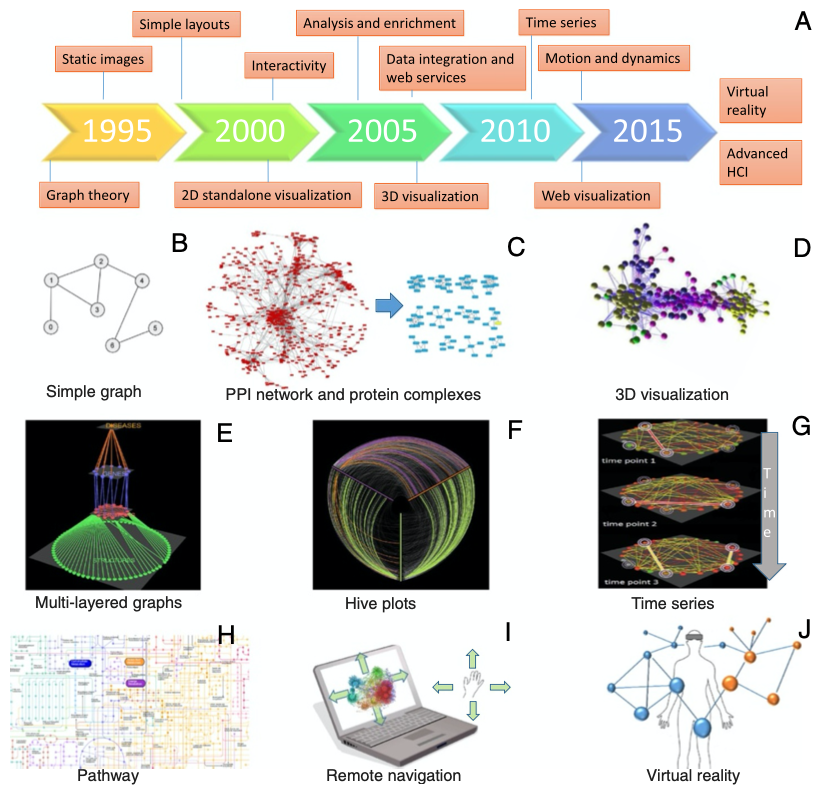
\includegraphics[width=\textwidth]{evolution_visualization}
    \caption{Visualization for network biology. a Undirected unweighted graph showing co-expression relationship between genes. b A 2D representation of a yeast protein-protein interaction network visualized in Cytoscape (left) and potential protein complexes 3D identified by the MCL algorithm from that network (right). c A 3D network of genes showing co-expression relationships. d A multilayered network integrating different types of data visualized by Arena3D. e A hive plot view of a network where nodes are mapped to and positioned on radially distributed linear axes. f Visualization of network changes over time. g Static picture showing part of lung cancer pathway. h Navigation of networks using hand gestures. i Integration and control of 3D networks using VR devices. Figure adapted\cite{pavlopoulos_malliarakis_papanikolaou_theodosiou_enright_iliopoulos_2015}.}
    \label{fig:network_biology_evolution}
\end{figure}%

We believe that virtual reality (VR) can offer new possibilities for visual inspection in large networks and for the inspection of patterns in these. Even though VR is still a field under exploration, it has been demonstrated that it help scientists work more effectively in fields like medicine \cite{Laver11}\cite{xia_ip_samman_wong_gateno_wang_yeung_kot_tideman_2001}\cite{brain_damage_rehab}, biology\cite{10.1093/bioinformatics/bti581}\cite{thorley_lawson_duca_shapiro_2008} and neuroscience\cite{bohil_alicea_biocca_2011}\cite{minderer_harvey_donato_moser_2016}, to  cite some examples. VR can be very powerful because it takes advantage of the way the human being perceives and analysis things. We have a great ability to discover patterns; however, we are biologically optimized to see the world and the patterns in 3 dimensions. Some of the advantages that VR has over non-VR approaches are the following:

\begin{enumerate}
  \item Visualization of networks in an immersive 3D space.
  \item Possibility to move around the virtual environment and visualize the network from different perspectives as in real life.
  \item Interaction with the the environment by using hand controllers or our hands.
  \item Integration of 2D interfaces in the virtual world that the user can interact with.
\end{enumerate}

We have implemented GeneNet VR, a virtual reality application for the visualization of 3-dimensional networks of genetic data. We have used up-to-date virtual reality techniques that we believe improve the visualization of this type of data structures. The techniques that we have used consist on: exploration of the network by moving around the virtual space, making it easier for the user to see the network from different perspectives; interaction with the network and the nodes to comprehend better the data and its associations; and the use of 2-dimensional user interfaces to manipulate the data for a easier pattern finding.

We saw that some of the interactions in GeneNet VR could have more impact in the performance of the application. This problem could escalate when using larger datasets. A high performance solution is desired so that the pattern exploration in the network is not affected.

\textbf{Thesis statement: } \emph{Virtual Reality techniques can be useful for the visualization of abstract networks and for the exploration of patterns in them}.

\section{Challenges and research problem}
This project focus mainly on solving the problem of visualization of high dimenasional data from the MIxT project by using virtual reality. Furthermore the application allows the user to interact with the network created from the data in the virtual environment. It also allows the user compare the blood and biopsy networks at the same time in order to finde relationship, which wasn't possible in the MIxT web application as this only allows the user to visualize one network at a time.

MIxT\cite{fjukstad_dumeaux_olsen_lund_hallett_bongo_2017} is a web application for bioinformaticians. Among other tools, it offers a network visualization of genes which are represented as nodes in the network and where the edges represent statistically significant correlation in expression between two nodes. This tool was used in a study\cite{dumeaux_fjukstad_interactions_tumor_blood} that identifies genes and pathways in the primary tumor that are tightly linked to genes and pathways in the systemic response of a patient with breast cancer.
When exploring a network in MIxT, it can be hard to understand the data and its relationships because there is too much data. This problem is easy to occur when there are too many node and edges. In figure \ref{fig:mixt_network} we can see an example of the network visualization from MIxT. As we can see in Figure \ref{fig:mixt_network1}, there are many nodes and relationships among them and when we zoom in in the network, it becomes very difficult to understand the data and the relationships as shown in in Figure \ref{fig:mixt_network_zoom}.

 The network is also in 2-dimensions and what we propose in this project is to use a virtual reality 3d visualization in order to cope better with this problem.

\begin{figure}[h!]
    \centering%
    \begin{subfigure}[t]{0.5\textwidth}
        \centering%
        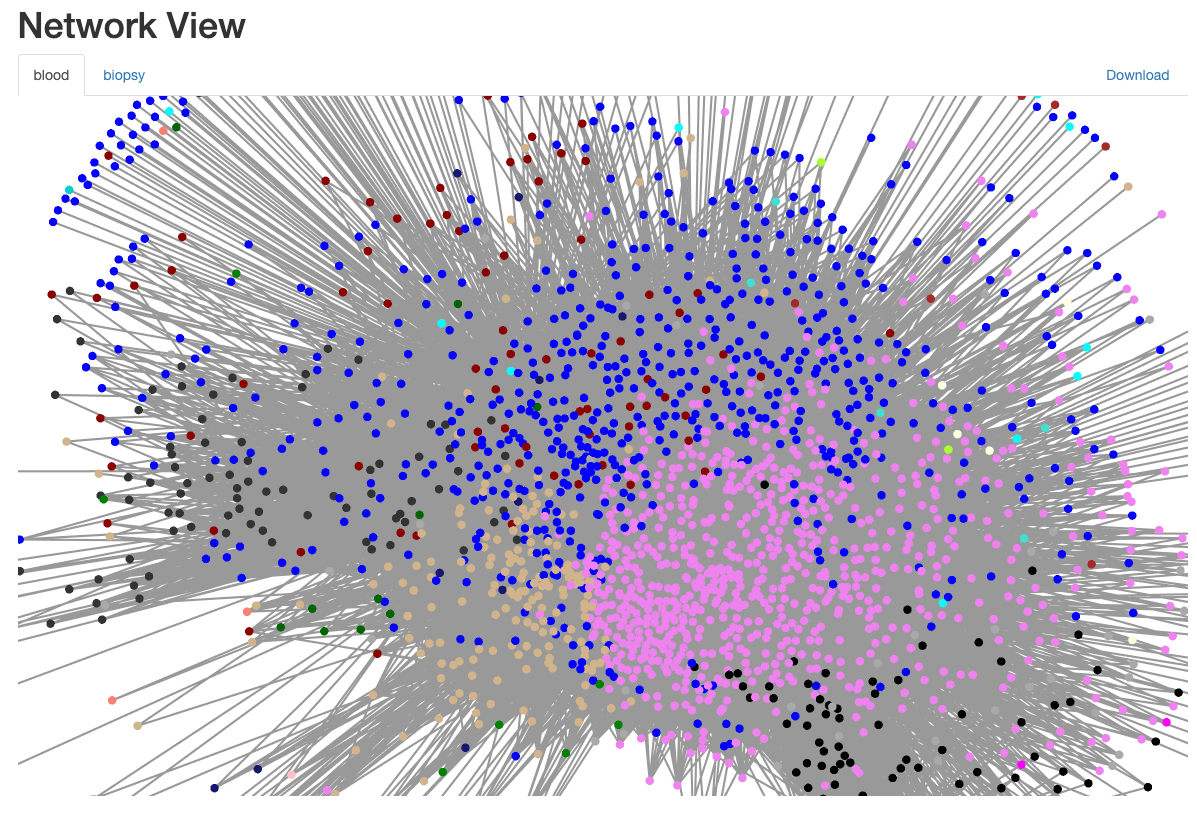
\includegraphics[width=\linewidth]{mixt_network1}
        \caption{Network with several modules.}
        \label{fig:mixt_network1}
    \end{subfigure}%
    \begin{subfigure}[t]{0.5\textwidth}
        \centering%
        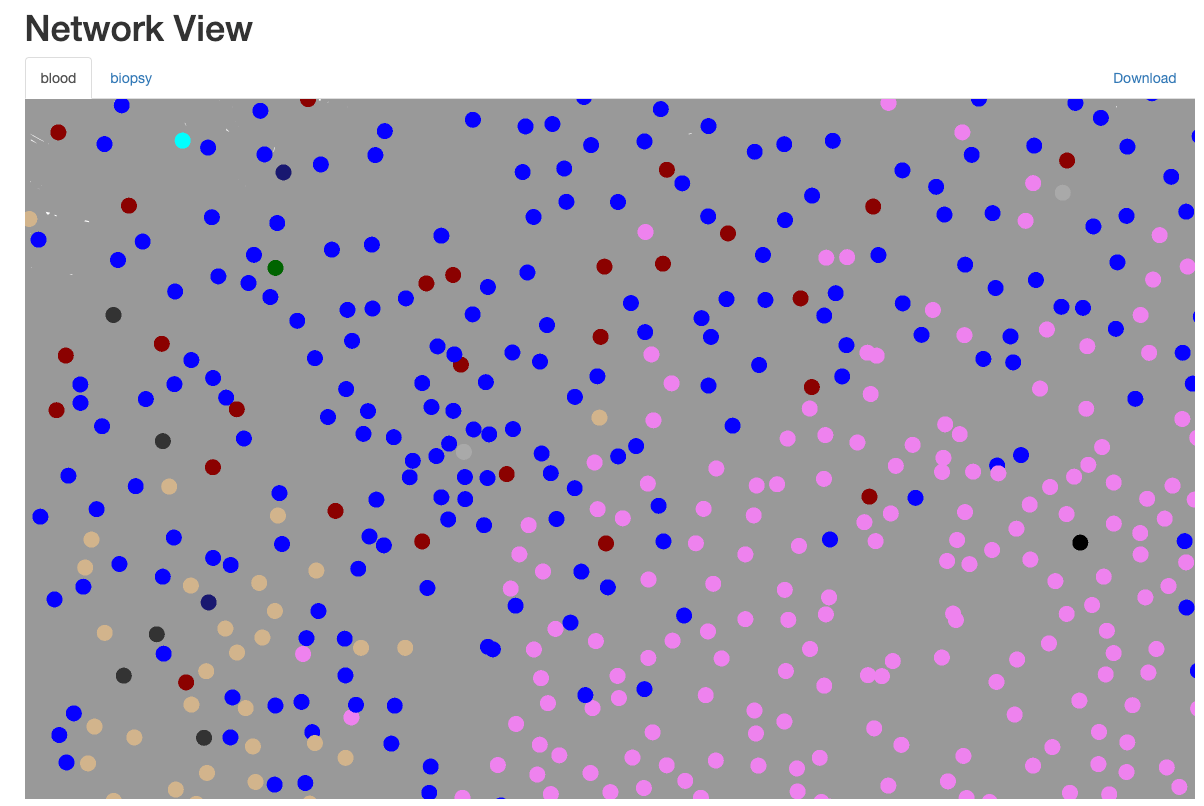
\includegraphics[width=\linewidth]{mixt_network2}
        \caption{Zoom in the network.}
        \label{fig:mixt_network_zoom}
    \end{subfigure}

    \caption{Network view of the MIxT application where nodes repsent genes and the modules are repsented by colors. Relationships are represented by grey lines that connect a gene with another one.}
    \label{fig:mixt_network}
\end{figure}

\section{Proposed solution}

\section{Significance and contribution}
This project contributes in the exploration of the possibilities that Virtual Reality offers for visualization of big data in bioinformatics.

\section{Outline}
